
\subsection{Gruppen, Ringe, Körper} \label{sec:3}
\begin{itemize}
\item Gegeben sei eine Menge $M$ und eine zweistellige Operation $\circ$ (d.h. Abb. von $M\times M$ in $M$)\\
Bezeichnung: $(M,\circ)$, analog $(M, \circ, *)$
\item Die Operation $\circ$ heißt \emph{kommutativ}, wenn $a \circ b= b \circ a $ für alle $a, b \in M$.
\item Die Operation $\circ$ heißt \emph{assoziativ}, wenn $(a \circ b) \circ c =a \circ (b \circ c)$ für alle  $a, b, c \in M$.
\end{itemize}

\paragraph{Def. 1:}\parskp
$(M,\circ)$ heißt \emph{Gruppe}, wenn gilt:
\begin{enumerate}
\item Die Operation $\circ$ ist assoziativ
\item Es gibt genau ein \emph{neutrales Element} $e\in M$ mit $a\circ e = e\circ a = a$ (für alle $a \in M$)
\item Es gibt zu jedem $a \in M$ genau ein \emph{inverses Element} $a^{-1}$ mit $a\circ a^{-1}=a^{-1}\circ a = e$
\item Eine Gruppe heißt \emph{ABELsch}, wenn zusätzlich folgendes gilt:\\
$\circ$ ist kommutativ
\end{enumerate}

\paragraph{Def. 2:}\parskp
$(M,\oplus,*)$ heißt \emph{Ring}, wenn gilt:
\begin{enumerate}
\item $(M, \oplus)$ ist eine ABELsche Gruppe.
\item Die Operation $*$ ist assoziativ.
\item Es gelten für beliebige $a,b,c\in M$:\\
$a*(b\oplus c)=(a*b)\oplus (a*c)\\
(a \oplus b) *c = (a*c) \oplus (b*c)$ \qquad (Distributivgesetze)
\item Ein Ring heiß \emph{kommutativer Ring}, wenn gilt:\\
$*$ ist kommutativ
\end{enumerate}

\paragraph{Def. 3:}\parskp
$(M, \oplus, *)$ heißt \emph{Körper}, wenn gilt:
\begin{enumerate}
\item $(M,\oplus, *)$ ist ein Ring \\
(mit dem neutralen Element $E_0$ für die Operation $\oplus$)
\item $(M\setminus \{E_0\}, *)$ ist eine ABELsche Gruppe\\
(mit dem neutralen Element $E_1$ für die Operation $*$)
\end{enumerate}

\subsection{Zahlentheorie}
\begin{itemize}
\item Eine natürliche Zahl $p>1$, die nurch durch $1$ und sich selbst teilbar ist heißt \emph{Primzahl}.
\item Jede natürliche Zahl $n>1$ ist entweder eine Primzahl, oder sie lässt sich als Produkt von Primzahlen schreiben.\\
Diese sogenannte \emph{Primfaktorzerlegung} ist bis auf die Reihenfolge der Faktoren eindeutig.
\end{itemize}

\paragraph{Def. 4:}\parskp
Zwei natürliche zahlen aus $\mathbb{N}^*$ heißen \emph{teilerfremd}, wenn sie außer $1$ keine gemeinsamen teiler besitzen.
\begin{itemize}
\item Es sei $a \in \mathbb{Z}$ und $m\in\mathbb{N}^*$. Dann gibt es eine eindeutige Darstellung der Gestalt $\boxed{a=q\cdot m + r}$ mit $\boxed{0\leq r < m}$ und $q \in \mathbb{Z}$.\\
Bezeichnung: $m$ … \emph{Modul} \qquad $r$ … (kleinste nichtnegative) \emph{Rest modulo m} ($r \equiv mod (a,m)$)
\item Zur Erinnerung: $a$ und $b$ seien ganze Zahlen, $m\in \mathbb{n}^*$, dann $a\equiv b (mod\; m)$ [$a$ kongruent $b\; modulo\; m$]\\
$\Leftrightarrow$ $a$ und $b$ haben den gleicher Rest $modulo\; m$\\
$\Leftrightarrow$ $a-b$ ist durch $m$ teilbar (d.h. $\exists k \in \mathbb{Z} \quad a-b = k\cdot m$)
\paragraph{Satz 1:} \parskp
Es sei $a \equiv b (mod\; m)$, $c\equiv d (mod\; m)$, dann gilt: $a+c \equiv b+d (mod \;m)$ und $a\cdot c \equiv b \cdot d (mod\; m)$ (d.h. in Summen und Produktenn darf jede Zahl durch einen beliebigen Vertreter der gleichen Restklasse ersetzt werden).
\subparagraph{Bsp. 1:} 
\begin{enumerate}[label=\alph*)]
\item $307+598 \equiv 1+(-2)\equiv -1 \equiv 5 (mod \; 6)$
\item $307\cdot 598 \equiv 1 \cdot (-2) \equiv -2 \equiv 4 (mod \; 6)$
\item $598^6 \equiv (-2)^6\equiv 64 \equiv 4 (mod \; 6)$
\end{enumerate}
\item Man wählt aus jeder Restklasse den kleinsten nichtnegativen Vertreter \\
$\curvearrowright$ Menge von Resten $modulo \; m$: $\mathbb{Z}_m:= \{0,1,...,m-1\}$ \\
$\curvearrowright$ „modulare Arithmetik“: Operation $\oplus$ und $\odot$ für Zahlen aus $\mathbb{Z}_m$ erklärbar, in dem für das Ergebnis jeweils der kleinste nichtnegative Rest $modulo \; m$ gewählt wird (vgl. Satz 1)\\
z.B. $\mathbb{Z}_7 = \{ 0,1,..., 6\}$, \quad $5\oplus 4=2$, da $5+4\equiv 9\equiv 2 (mod \; 7)$ \quad $5\odot 6=2$, da $5\cdot 6\equiv 30 \equiv 2 (mod \;7)$\smallskip\\
Falls keine Verwechselung zu befürchten ist, wird die übliche Schreibweise $+$ und $\cdot$ anstelle von $\oplus$ und $\odot$ verwendet.
\end{itemize}

\paragraph{Def. 5:} \parskp
Wenn es zu $c \in \mathbb{Z}_m$ eine Zahl $d\in \mathbb{Z}_m$ gibt, mit $c\cdot d \equiv 1 (mod \; m)$ (bzw. $c\odot d \equiv 1$), so heißt $d$ die \emph{(multiplikative) modulare Inverse} zu $c$ in $\mathbb{Z}_m$.\\
Bezeichnung: $d=c^{-1}$
\subparagraph{Bsp. 2:} \parskp
$c=3 \in \mathbb{Z}_7$, wegen $3 \cdot 5 \equiv 1 (mod \; 7)$ ist (in $\mathbb{Z}_7$) $3^{-1}=5$.
\subparagraph{Satz 2:} Zu $a \in \mathbb{Z}_m, a \not = 0$, gibt es genau dann eine modulare Inverse in $\mathbb{Z}_m$, wenn $a$ und $m$ teilerfremd sind ($ggT(a,m)=1$).
\subparagraph{Satz 3:} Es sei $p$ eine Primzahl. Dann ist $(\mathbb{Z}_m, \oplus, \odot)$ ein Körper.\\
Bemerkung: Falls $m$ keine Primzahl ist, so ist $(\mathbb{Z}_m, \oplus, \odot)$ ein kommutativer Ring.
\subparagraph*{EUKLIDischer Algorithmus}
\begin{itemize}
\item Verfahren zur Ermittlung des größten gemeinsamen Teilers $t$ zweier positiver natürlicher Zahlen, $t=ggT(a,b)$.
\item In erweiterter Form bietet der Algorithmus eine Möglichkeit zur Bestimmung  der modularen Inversen von $a$ zum Modul $m$ (mit $a<m$ und $a,m$ teilerfremd).
\end{itemize}

\subparagraph{Satz 4:} (EUKLIDischer Algorithmus)\\
Es seien $a,b \in \mathbb{N}^*, a>b$. Man bildet die endliche Folge \\
$r_0:= b, \; r_1=mod \;(a,b), \;r_2 = mod \; (r_0,r_1),...,\;r_n = mod \; (r_{n-2}, r_{n-1})$, Abbruch falls $r_n=0$.\\
In diesem Fall gist $\boxed{ggT(a,b)=r_{n-1}}$ (letzter nicht verschwindender Rest).\\
Bezeichnung: $j$-te Division ... $\boxed{r_{j-2}:r_{j-1}= q_j\text{ Rest } r_j}$ ($j=1,...,n$) (dabei $r_1:=a$).

\subparagraph{Satz 5:}  (erweiterter EUKLIDischer Algorithmus)\\
Zusätzlich zur Folge $(r_n)$ aus Satz 4 bilde man die Folgen \\
$x_0=0,\; x_1=1, \; x_2 = x_0 - q_2x_1, ...,\; x_j=x_{j-2}-q_jx_{j-1}\quad (j\leq n-1)$ und\\
$y_0=1, \; y_1=-q_1, \; y_2=y_0- q_2 y_1, ... ,\; y_j=y_{j-2}-q_jy_{j-1}\quad (j \leq n-1)$\\
Dann gilt für alle $j=0, ..., \; n-1$: $\boxed{r_j=x_j\cdot a + y_j \cdot b}$\\
Insbesondere gilt $\boxed{ggT(a,b) = x_{n-1}\cdot a + y_{n-1}\cdot b}$
\subparagraph{Diskussion:}
\begin{enumerate}
\item Der Sinn der erweiterten EUKLIDischen Algorithmus besteht darin, in jedem Schrit den \emph{Divisionsrest $r$ als linearkombination von $a$ und $b$ mit ganzzahligen Koeffizienten $x$ und $y$} darzustellen: $r=x\cdot a + y\cdot b$\\
Der Mechanismus wird am besten im Rechenschema des nachfolgenden Bsp. 4 deutlich.
\item  Sind $c$ und $m$ teilerfremd, $1\leq c < m$, d.h. $ggT(m,c)=1$, so erhält man mit dem erweiterten EUKLIDischen Algorithmus ($a=m, b=c$) eine Darstellung in der Form $\boxed{1=x\cdot m+ y\cdot c}$.\\
$\curvearrowright y\cdot c \equiv 1 (mod\; m)$ und damit $c^{-1}\equiv y (mod\; m)$ (für die modulare Inverse muss eventuell noch der in $\mathbb{Z}_m$ liegende, zu $y$ kongruente, Wert gebildet werden!).
\end{enumerate}

\subparagraph{Bsp. 3:} \parskp
Man ermittle den größten gemeinsamen Teiler $t$ sowie das kleinste gemeinsame Vielfache $v$ der Zahlen $132$ und $84$.
\begin{itemize}
\item Es genügt der „einfache“ Algorithmus:
\begin{align*}
132:84 &= 1\text{ Rest } 48\\
84:48 &= 1\text{ Rest } 36\\
48:36 &= 1\text{ Rest } 12 \quad \curvearrowright t = ggT (132,84) = \resultul{12}\\
36:12 &= 3\text{ Rest } \boxed{0} \curvearrowright \text{ Ende.}\\
\end{align*}
\item $v=\frac{a \cdot b}{t}=\frac{132\cdot 84}{12}=\resultul{924}=kgV (132,84)$
\end{itemize}

\subparagraph{Bsp. 4:} \parskp
Man ermittle die modulare Inverse von $\overbrace{11}^b$ zum Modul $\overbrace{25}^a$. \medskip\\
\begin{tabular}{r l | l | r l}
				&				&						&	$11$&$=0 \cdot 25 + 1 \cdot 11$ (1)\\
$25:11 $&$= 2 \text{ Rest }  3$	&	$3=25-2 \cdot 11$	&	$3 $&$= 1 \cdot 25 - 2 \cdot 11$ (2)\\
$11: 3 $&$= 3 \text{ Rest } 2$		&	$2= 11-3 \cdot 3$	&	$2 $&$= -3 \cdot 25 + 7 \cdot 11$ (3)\\
$3:2 $&$= 1 \text{ Rest } 1$		&	$1 = 3-2$			&	$\boxed{1} $&$= 4 \cdot 25 - 9 \cdot 11$\\
$2 : 1 $&$= 2 \text{ Rest }  0$	&						& &\\
\end{tabular} \medskip\\
$\curvearrowright (-9) \cdot 11 \equiv 1 (mod \; 25)\\
\curvearrowright 11^{-1} \equiv -9 \equiv 16 (mod \; 25)$, die Inverse von $11$ in $\mathbb{Z}_{25}$ ist $16$.\\
Zu den Schritten:
\begin{itemize}
\item [(1)] $b=0 \cdot a + 1 \cdot b$
\item [(2)] mittleres Feld als Linearkombination
\item [(3)] ab hier Rechnung links spaltenweise durchführen, dabei Faktoren $a$ und $b$ beibehalten. 
\end{itemize}
\subsubsection*{EULERsche $\varphi$-Funktion, Satz von EULER}
\paragraph{Def. 6:} \parskp
Es sei $n \in \mathbb{N}^*$. Dann \emph{EULERsche $\varphi$-Funktion}:

$\varphi(n):=$ Anzahl der zu $n$ teilerfremden Elemente aus $\{1,2,...,n\}$.
Eigenschaften der $\varphi$-Funktion:
\begin{itemize}
\item Es sei $p$ eine Primzahl, dann ist $\boxed{\varphi(p)=p-1}$, $\boxed{\varphi(p^k)=p^{k-1}(p-1)} \; (k \in \mathbb{N}^*$
\item Falls $ggT (m, n) =1$, so gilt $\varphi (m\cdot n) = \varphi (m) \cdot \varphi (n)$.
\item Speziell: $n=p\cdot q $ ($p,q$ Primzahlen), dann $\boxed{\varphi(n)=(p-1)\cdot (q-1)}$ (1).
\end{itemize}
\subparagraph{Satz 6:} (Satz von EULER)\\
Es sei $ggT(a,n)=1$, dann gilt:\\
$\boxed{a^{\varphi(n)}\equiv 1 (mod \; n)}$ (2).

\subsubsection*{RSA-Verschlüsselung}
\begin{itemize}
\item Die Formeln (1) und (2) [siehe oberhalb] bilden die Grundlage für die sogenannte RSA-Ver\-schlüsselung (RIVES, SHAMIR, ADLEMAN - 1978)
\item Schlüsselerzeugung:
\begin{enumerate}
\item Man wählt (in der Praxis sehr große) Primzahlen $d$ und $q$.
\item $n:= p \cdot q$, $m:= \varphi (n) \overset{(1)}{=} (p-1)(q-1)$
\item $e$ wird so gewählt, dass $ggT(e,m)=1$
\item $d:= e^{-1} (mod \; m)$ (modulare Inverse)
\item $(n,e)$ … öffentlicher Schlüssel\\
$(n,d)$ … geheimer Schlüssel (geheim ist nur $d$)\\
$p$, $q$ und $m$ werden nicht mehr benötigt, bleiben aber geheim!
\end{enumerate}
\item Verschlüsselung: \\
Klartext $a$ teilerfremd zu $n$ verschlüsseln mit $e$, d.h. $b:\equiv a^e (mod \; n)$ bilden ($b$ … Geheimtext)
\item Entschlüsselung: \\
Der Empfänger und Besitzer des geheimen Schlüssels bildet $b^d (mod \; m)$ und erhält $b^d\equiv a (mod \; n)$ denn $b^d\equiv (a^e)^d \equiv a^{ed}\equiv a ^{1+k\cdot m}\equiv a\cdot \underset{\equiv 1 \text{ wegen Satz 5}}{\left( a^{\varphi(n)}\right)}^k\equiv a (mod \; n)$.
\item Praktische Durchführung vgl Übungsaufgabe 2.4
\end{itemize}

\subsection{Reelle Zahlen}

$\mathbb{R}$ … Menge der reellen Zahlen.\\
Auf $\mathbb{R}$ existiert eine algebraische Struktur und eine Ordnungsstruktur.

\subsubsection{Algebraische Struktur}
$(\mathbb{R}, + ,\cdot)$ mit den arithmetischen Operationen $+$ (Addition) und $\cdot$ (Multiplikation) ist ein Körper.
\paragraph{Def. 7:}
\begin{enumerate}[label=\alph*.)]
\item $\boxed{0! := 1, \; n!=n\cdot (n-1)!}$ mit $n\in \mathbb{N}^*$ \emph{Fakultät} (rekursive Funktion)
\item Sei $\alpha \in \mathbb{R}, k\in \mathbb{N}^*$, dann sei $\boxed{\nok{\alpha}{0}:=1, \nok{\alpha}{k}:= \frac{\alpha}{k}\nok{\alpha-1}{k-1}}$ Binominalkoeffizient $\alpha$ über $k$.\\
d.h. $\boxed{\nok{\alpha}{k}= \frac{\alpha(\alpha-1)(\alpha-2)...(\alpha-k-1)}{k!}}$
\end{enumerate}

\subparagraph{Diskussion:}
\begin{enumerate}
\item Für $k, n \in \mathbb{N}, \; 0 \leq k \leq n$ gilt $\boxed{\nok{n}{k}=\nok{n}{n-k}=\frac{n!}{k!(n-k)!}}$
\item Für $k \in \mathbb{N}, \alpha \in \mathbb{R}$ gilt $\boxed{\nok{\alpha}{k}+\nok{\alpha}{k+1}=\nok{\alpha+1}{k+1}}$
\item \emph{Binomischer Lehrsatz}: $(a+b)^k=\sum_{k=0}^n \nok{n}{k} a^{n-k} \cdot b^k=a^n+n\cdot a^{n-1} \cdot b + \nok{n}{2}a^{n-2}\cdot b^2+...+b^n$\\
\emph{Pascalsches Dreieck}:
\begin{tabular}{c c c c c c c c c c c r}
   &   &   &   &   & 1 &   &   &   &   &   & \textcolor{red}{$n=0$} \\
   &   &   &   & 1 &   & 1 &   &   &   &   & \textcolor{red}{$1$} \\
   &   &   & 1 &   & 2 &   & 1 &   &   &   & \textcolor{red}{$2$} \\
   &   & 1 &   & 3 &   & 3 &   & 1 &   &   & \textcolor{red}{$3$} \\
   & 1 &   & 4 &   & 6 &   & 4 &   & 1 &   & \textcolor{red}{$4$} \\
 1 &   & 5 &   & 10&   & 10&   & 5 &   & 1 & \textcolor{red}{$5$} \\

\end{tabular}
(Spalte $\widehat{=}k$ in $\nok{n}{k}$)
\end{enumerate}

\paragraph{Stellenwertsysteme:} \label{Stellenwertsysteme}
\begin{itemize}
\item Es sei $k>1$ eine natürliche Zahl (die sogenannte Basis)
\item $x = (\underbrace{x_p x_{p-1}...x_1x_0}_{\text{Vorkomma}},\;\underbrace{x_{-1}x_{-2}...x_{-q}}_{\text{Nachkomma}})_b\\
:= \underbrace{x_p\cdot b^p+x_{p-1}\cdot b^{p-1}+...+x_1\cdot b^1+x_0\cdot b^0}_{\text{Vorkomma}}+\underbrace{x_{-1}\cdot b^{-1}+x_{-2}\cdot b^{-2}+...+x_{-q}\cdot b^{-q}}_{\text{Nachkomma}}$\\
heißt Darstellung zur Basis b (*).
\end{itemize}

\subparagraph{Bsp. 5:}
\begin{itemize}
\item $b=2$ … \emph{Dual- oder Binärsystem} (Ziffern $\{0,1\}$)
\item $b=3$ … Trialsystem
\item $b=10$ … \emph{Dezimalsystem}
\item $b=16$ … \emph{Hexadezimalsystem} (Ziffern $\{0,1,2,...,9,\underset{10}{A},\underset{11}{B},\underset{12}{C},\underset{13}{D},\underset{14}{E},\underset{15}{F}\}$
\end{itemize}
z.B. $(47)_{10}=(101111)_2=(1202)_3=(57)_8=(2F)_{16}$
\paragraph{Übergang von einem Ziffernsystem zu einem anderen}\parskp
z.B. $p=3,\; q=2$
\begin{align*}
x&=x_3b^3+x_2b^2+x_1b^1+x_0+x_{-1}b^{-1}+x_{-2}b^{-2}\\
&= (x_3b^2+x_2x^1+x_1)b+x_0+(x_{-1}+x_{-2}b^{-1})b^{-1}\\
&=((x_3b^1+x_2)b+x_1)b+x_0+(x_{-1}+x_{-2}b^{-1})b^{-1}
\end{align*}
Grundlage: fortgesetztes Klammern:
\begin{align*}
x&=((....((x_p b+x_{p-1})b+x_{p-2})b+...+x_2)b+x_1)b+x_0+\\
&\qquad((...(x_{-q}b^{-1}+x_{-(q-1)})b^{-1}+...+x_{-2})b^{-1}+x_{-1})b^{-1}
\end{align*} (**)
\subparagraph{Bsp. 6:} Übergang Dezimalsystem $\rightarrow$ anderes System
\begin{itemize}
\item ganzer Teil: fortgesetzte Division durch $b$ und Restabspaltung liefert $b$-Ziffern in der Reihenfolge $x_0,x_1,x_2,...$
\item gebrochener Teil: fortgesetzte Multiplikation mit $b$ und Abspaltung des ganzzahligen Anteils liefert $b$-Ziffern in der Reihenfolge $x_{-1},x_{-2},...$
\end{itemize}
z.B. Dezimalsystem $\rightarrow$ Hexadezimalsystem ($b=16$)\\
$x=435,9$\\
ganzer Teil:\\
\begin{tabular}{r c l l}
$435:16=$ & $27$ & Rest $3$ &  $\rightarrow x_0$\\
$27:16=$ & $1$ & Rest $11$ &  $\rightarrow x_1$\\
$1:16=$ & $\boxed{0}$ & Rest $1$ &  $\rightarrow x_2$\\
\end{tabular}\\
gebrochener Teil: \\
\begin{tabular}{r c l l}
$0,9 \cdot 16=$ & $0.4$ & $+14$ & $\rightarrow x_{-1}$\\
$0,4 \cdot 16=$ & $\boxed{0.4}$ & $+6$ & $\rightarrow x_{-2}$ (Periode, da gleicher „Nachkommarest“)\\
\end{tabular}\\
$\curvearrowright x=(1B3,E\overline{6})_{16}$

\subparagraph{Bsp. 7:} Übergang anderer Systeme $\rightarrow$ Dezimalsystem\\
Entweder direkte Auswertung von (*) (v.a. beim Dualsystem $\rightarrow$ Addition von 2er-Potenzen) \emph{oder} Klammern in (**) von innen nach außen berechnen (zweckmäßig HORNER-Schema).
\begin{itemize}
\item ganzer Teil: beginnend mit $x_p$\\
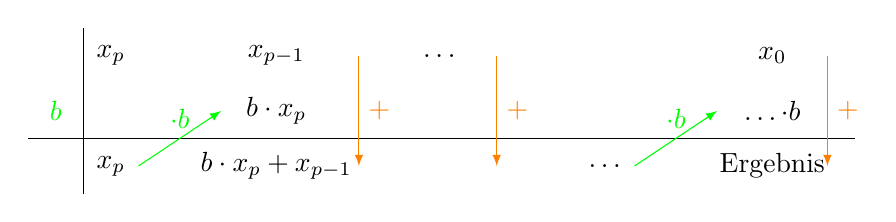
\begin{tikzpicture}[scale=.7]
\node at (0,2) {$x_p$};
\node at (0,0) {$x_p$};
\node at (3,2) {$x_{p-1}$};
\node at (3,1) {$b\cdot x_p$};
\node at (3,0) {$b\cdot x_p+x_{p-1}$};
\node at (6,2) {…};
\node at (9,0) {…};
\node at (12,2) {$x_0$};
\node at (12,0) {Ergebnis};

\draw (-0.5,2.5) -- (-0.5,-0.5);
\draw (-1.5,0.5) -- (13.5,0.5);
\node [green] at (-1,1) {$b$};
\draw [-latex, green] (0.5,0) -- (2,1) node[pos=.5, above]{$\cdot b$};
\draw [-latex, green] (9.5,0) -- (11,1) node[pos=.5, above]{$\cdot b$};

\draw [-latex, orange] (4.5,2) -- (4.5,0)node[pos=.5, right]{$+$};
\draw [-latex, orange] (7,2) -- (7,0)node[pos=.5, right]{$+$};
\draw [-latex, orange] (13,2) -- (13,0)node[pos=.5, right]{$+$};
\node at (12,1) {…$\cdot b$};
\end{tikzpicture}
\item gebrochener Teil: beginnend mit $x_{-q}$\\
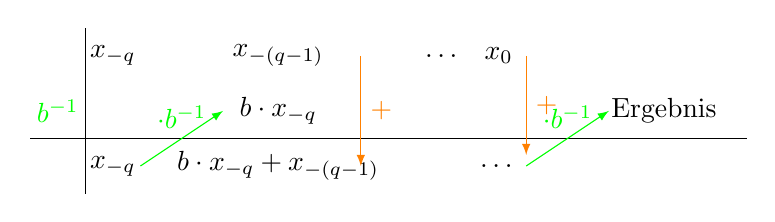
\begin{tikzpicture}[scale=.7]
\node at (0,2) {$x_{-q}$};
\node at (0,0) {$x_{-q}$};
\node at (3,2) {$x_{-(q-1)}$};
\node at (3,1) {$b\cdot x_{-q}$};
\node at (3,0) {$b\cdot x_{-q}+x_{-(q-1)}$};
\node at (6,2) {…};
\node at (7,0) {…};
\node at (7,2) {$x_0$};
\node at (10,1) {Ergebnis};

\draw (-0.5,2.5) -- (-0.5,-0.5);
\draw (-1.5,0.5) -- (11.5,0.5);
\node [green] at (-1,1) {$b^{-1}$};
\draw [-latex, green] (0.5,0) -- (2,1) node[pos=.5, above]{$\cdot b^{-1}$};
\draw [-latex, green] (7.5,0) -- (9,1) node[pos=.5, above]{$\cdot b^{-1}$};

\draw [-latex, orange] (4.5,2) -- (4.5,0)node[pos=.5, right]{$+$};
\draw [-latex, orange] (7.5,2) -- (7.5,0.2)node[pos=.5, right]{$+$};
\end{tikzpicture}
\end{itemize}
$x=(1E2,B8)_{16}$\\
ganzer Teil:\\
\begin{tabular}{c | c c c}
 & $1$  &  $14$  & $2$\\
 $16$  &   & $16$  & $480$\\
 \hline
  & $1$ & $30$ & $\boxed{482}$\\

\end{tabular}\\
gebrochener Teil:\\
\begin{tabular}{c | c c c}
 & $8$  &  $11$  & *\\
 $\frac{1}{16}=0,0625$  &   & $0,5$  & $\boxed{0,71875}$\\
 \hline
  & $8$ & $11,5$ & \\
\end{tabular}\\
$\curvearrowright x=\resultul{482,71875}$

\subparagraph{Bsp. 8:} Hexadezimalsystem $\leftrightarrow$ Dualsystem\\
4 Dualziffern entsprechen einer Hexadezimalziffer ($2^4=16$) $\curvearrowright$ 4er Gruppen von Dualziffern ab Komma bilden.
\begin{enumerate}[label=\alph*.)]
\item $(A8C,B2)_{16}=(1010 \; 1000 \; 1100, \; 1011 \; 1011 \; 001(0))_2$
\item $((0)110\; 1110, \; 101(0))_2 = (6E,A)_{16}$
\end{enumerate}

\subsubsection{Zahlendarstellung im Computer}

\begin{enumerate}
\item Ganze Binärzahlen in Zweierkomplementdarstellung ($n$ Bit, meist $n=8,16,32,64$)
\begin{itemize}
\item Bsp.: $n=8 \qquad (100)_{^10}=(64)_{16}$\\
\begin{tabular}{|c | c | c |c | c | c |c | c |}
\hline
\textcolor{red}{0} & 1 &1&0&0&1&0&0\\
\hline
$2^7$&$2^6$&$2^5$&$2^4$&$2^3$&$2^2$&$2^1$&$2^0$\\
\hline
\end{tabular}\\
\textcolor{red}{MSB}: most siginficant bit\\
(LSB: least significant bit)
\item Um auch negative Zahlen darstellen zu können, wird das MSB als Vorzeichen reserviert. Negative Zahlen $-a$ ($1\leq a \leq 2^{n-1}$) werden im sogenannten Zweierkomplement $\overline{a}:=2^n-a$ dargestellt ($\curvearrowright \overline{a}\geq 2^{n-1} \curvearrowright MSB =1$)
\item Nightnegtavie Zahlen $0\leq a \leq 2^{n-1}-1$ werden unverändert dargestellt ($MSB=0$)
\item Damit Darstellung ganzer Zahlen von $-2^{n-1}$ bis $2^{n-1}-1$ (Anzahl $2^n$) möglich, $n=8: -128 bis 127$.
\item Umwandlung negativer Zahlen $\rightarrow$ Zweierkomplement
\subparagraph{Bsp. 9:} $n=8$, umzuwandeln sei $-100$ (dezimal)\\
zwei Möglichkeiten:
\begin{enumerate}[label=\arabic*.)]
\item  (für die Handrechnung): $\overline{100}=\underbrace{2^8}_{=256}-100=\underbrace{156}_{(9C)_{16}}=$\begin{tabular}{|c|c c c|c c c c|}
\hline
\textcolor{red}{$1$}&$0$&$0$&$1$&$1$&$1$&$0$&$0$\\
\hline
\end{tabular}\\
\emph{Bemerkung}: Das Zweierkomplement der positiven Zahl $100$ ist die positive Zahl $156=\overline{100}$, diese wird wegen $MSB=1$ als negative Zahl $-100$ interpretiert.
\item (am schnellsten): Rechts (beim LSB) beginnend alle Ziffern bis einschließlich der ersten $1$ übernehmen (unverändert lassen), für alle höherwertigen Ziffern $Z$ das \emph{Einerkomplement} $1-z$ bilden:\\
$(100)_{10}=$\begin{tabular}{|c|c c c|c c c c|}
\hline
$0$&$1$&$1$&$0$&$0$&$1$&$0$&$0$\\
\hline
\end{tabular}\\
\begin{tabular}{|c|c c c|c c c c|}
\hline
\textcolor{red}{$1$}&\textcolor{red}{$0$}&\textcolor{red}{$0$}&\textcolor{red}{$1$}&\textcolor{red}{$1$}&\textcolor{green}{$1$}&\textcolor{green}{$0$}&\textcolor{green}{$0$}\\
\hline
\end{tabular} $=(\overline{100})_{10}=(156)_2$\\
Rückumwandlung (Zahl mit $MSB=1 \rightarrow$ neg. Zahl) analog:\\
$\overline{156}=256-156=100\rightarrow \resultul{-100}$\\
Die Subtraktion wird damit auf die Addition des Zweierkomplements zurückgeführt.
\end{enumerate}
\subparagraph{Bsp. 10:} $a=64-100=64+(-100)$
\begin{align*}
64=2^6 &= 0100 \, 0000\\
-100 &= 1001 \, 1100 \quad +\\
Summe &= \textcolor{red}{1}101\, 1100 \quad \text{\textcolor{red}{Ergebins negativ}}\\
36 &= 0010\, 0100 \quad \text{dargestellst ist aber }\overline{z}=2^n-z
\end{align*}
$\curvearrowright$ Ergebnis: $a=-36=-z$\\
Ein \emph{Überlauf} (Ergebnis $\geq 2^{n-1}$ oder $<-2^{n-1}$) ensteht in folgenden Fällen ($\rightarrow$ ERROR!)
\begin{tabular}{r | c |c |c l}
 & $a$ & $b$ & $a+b$ & \\
 \hline
 MSB & 0 & 0& \textcolor{red}{1} & ($MSB = 0$ erwartet!)\\
 \hline 
 MSB & 1 & 1& \textcolor{red}{0} & ($MSB = 1$ erwartet!)\\
\end{tabular}\\
Bemerkung: Für die Handrechnung (z.B. $2-5=:a$) kleinere zahl von größerer Subtrahieren $a=-(5-2)$, dabei genügt es für $n$ die Binärstellenzahl des Minuenden $(5)_{10}=(101)_2$ also $n=3$  zu verwenden. Es wird dabei ausschließlich mit nicht-negativen Zahlen gerechnet ($0,1,...,2^n-1$):\\
$(5-2)_{10}=((5+\textcolor{red}{2^n}-2)-\textcolor{red}{2^n})_{10}=(5+\overline{2}-\textcolor{red}{2^n})_{10}$\\
$(2)_{10}=(010)_2 \curvearrowright \overline{2}=(110)_2$\\
$(5)_{10}=(101)_2$\\
\begin{tabular}{r l}
$5$:& $101$\\
$\overline{2}$:& $110 \quad +$\\
$\textcolor{red}{1}$& $011$
\end{tabular}\\
\textcolor{red}{vordere Stelle $2^n$ ignorieren}\\
$\curvearrowright 5-3=3=(011)_2 \curvearrowright \resultul{a=-3}$
\end{itemize}
\item Gleitkommasysteme\\
$\boxed{x=v\cdot m \cdot b^e}$ dabei
\begin{itemize}
\item $v=(-1)^V$ … \emph{Vorzeichen} $\begin{cases}
V= 0 \quad \text{positive Zahl}\\
V=1 \quad \text{negative Zahl}
\end{cases}$
\item $m$ … \emph{Mantisse}, Stellenzahl $p$, die Mantisse heißt \emph{normalisiert} falls sie folgende Gestalt besitzt:\\
 $m_1, m_2, ..., m_p$ oder $0, m_1, m_2, ..., m_p$ mit $m\not = 0$. Dabei sind  $m_1, m_2, ..., m_p$ die Ziffern zur Basis $b$.
\item $e$ … \emph{Exponent}, ganzzahlig $e_{min}\leq e \leq e_{max}$.
\end{itemize}
In jedem Gleitkommasystem sind nur endlich viele Zahlen darstellbar, die Menge der reellen zahlen ist aber überabzählbar (unendlich).\\
Gleitkommazahlen liegen auf der Zahlengeraden diskret verteilt (fester Exponent $\curvearrowright$ gleiche Abstände, wächst Exponent um $k$, so wachsen die Abstände auf $b^k$-fache!)\\
Veranschaulichung für $b=10$, Mantissenlänge $p=1$:\\
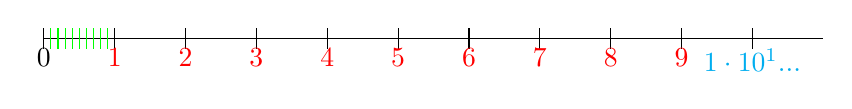
\begin{tikzpicture}[scale=0.9]
\draw (0,0) -- (11,0);
\draw (0,0) node[below]{0};
\draw (0,0.15)--(0,-0.15);
\draw (1,0.15)--(1,-0.15);
\draw (2,0.15)--(2,-0.15);
\draw (3,0.15)--(3,-0.15);
\draw (4,0.15)--(4,-0.15);
\draw (5,0.15)--(5,-0.15);
\draw (6,0.15)--(6,-0.15);
\draw (7,0.15)--(7,-0.15);
\draw (8,0.15)--(8,-0.15);
\draw (9,0.15)--(9,-0.15);
\draw (10,0.15)--(10,-0.15);
\draw (1,0) node[below]{\textcolor{red}{1}};
\draw (2,0) node[below]{\textcolor{red}{2}};
\draw (3,0) node[below]{\textcolor{red}{3}};
\draw (4,0) node[below]{\textcolor{red}{4}};
\draw (5,0) node[below]{\textcolor{red}{5}};
\draw (6,0) node[below]{\textcolor{red}{6}};
\draw (7,0) node[below]{\textcolor{red}{7}};
\draw (8,0) node[below]{\textcolor{red}{8}};
\draw (9,0) node[below]{\textcolor{red}{9}};

\draw[green] (0.1,0.15)--(0.1,-0.15);
\draw[green] (0.2,0.15)--(0.2,-0.15);
\draw[green] (0.3,0.15)--(0.3,-0.15);
\draw[green] (0.4,0.15)--(0.4,-0.15);
\draw[green] (0.5,0.15)--(0.5,-0.15);
\draw[green] (0.6,0.15)--(0.6,-0.15);
\draw[green] (0.7,0.15)--(0.7,-0.15);
\draw[green] (0.8,0.15)--(0.8,-0.15);
\draw[green] (0.9,0.15)--(0.9,-0.15);


\draw (10,0) node[below]{\textcolor{cyan}{$1\cdot 10^1$...}};
\end{tikzpicture}\\
\emph{Exponent} 0: $1\cdot 10^{\textcolor{red}{0}}, 2\cdot 10^{\textcolor{red}{0}}, ... , 9\cdot 10^{\textcolor{red}{0}}$\\
\emph{Exponent} -1: $1\cdot 10^{\textcolor{green}{-1}}, 2\cdot 10^{\textcolor{green}{-1}}, ... , 9\cdot 10^{\textcolor{green}{-1}}$\\
\emph{Exponent} 1: $1\cdot 10^{\textcolor{cyan}{1}}, 2\cdot 10^{\textcolor{cyan}{1}}, ... , 9\cdot 10^{\textcolor{cyan}{1}}$\\
\emph{Rundung}: Zahlen, die nicht in diesem „Raster“ enthalten sind, werden auf dei nächstgelegene darstellbare Gleitkommazahl gerundet. Falls die Zahl genau in der Mitte zwischen zwei darstellbaren Zahlen liegt, wird auf die gerade Zahl gerundet (Bsp. $3,75 \rightarrow 3,8$ oder $4,65 \rightarrow 4,6$ bei Rundung auf eine Stelle nach dem Komma).
\paragraph{Numerische Probleme beim Rechnen mit Gleitkommazahlen}
\begin{itemize}
\item Kommutativ-, Assoziativ- und Distributivgesetze gelten im allgemeinen nicht mehr. Ursachen sind bspw. Ziffernauslöschung bei der Subtraktion fast gleicher Zahlen, Addition oder Subtraktion von Zahlen unterschiedlicher Größenordnung.
\subparagraph{Bsp. 11:}
\begin{enumerate}[label=\arabic*.)]
\item Man berechne $(a+b)+c$ und $a+(b+c)$ in einem System mit 3-Stelliger Mantisse:\\
$a=3,73\cdot 10^6$, $b=-3,71\cdot 10^6$ und $c=6,42\cdot 10^3$
\begin{itemize}
\item $a+b= 0,02\cdot 10^6=2,00 \cdot 10^4$ (Normalisierung)\\
$c=0,642\cdot 10^4=0,64\cdot 10^4$ (Exponentenangleichung und Rundung)\\
$(a+b)+c=2,64\cdot 10^4=\resultul{26400}$
\item $c=0,00642\cdot 10^6=0,01\cdot 10^6$ (Exponentenangleichung und Rundung)\\
$b+c=-3,,70\cdot 10^6$\\
$a+(b+c)=0,03\cdot 10^6=3,00\cdot 10^4 = \resultul{30000}$
\item exakter Wert: $a+b+c = \resultul{26420}$
\end{itemize}
\item Aufgabe der numerischen Mathematik ist es, die unvermeidlichen Genauigkeitsverluste beim Rechnen mit Maschinenzahlen durch optimale Organisation (Reihenfolge) der Rechnung und Fehleranalyse in Grenzen zu halten.
\end{enumerate}
\end{itemize}
\item Gleitkommaformat IEEE 754 (single precision, 32 Bit)\\
$x=v\cdot m \cdot b^e=(-1)^{\torange{V}}\cdot 1, \tblue{m_2\,m_3...m_24}\cdot 2^{\tred{E}-B}$ ($b=2$, Binärsystenm)
\begin{itemize}
\item Vorzeichen $V=0\curvearrowright$ positiv, $V=1\curvearrowright$ negativ (1 Bit)
\item Mantisse $m_1$ im Binärsystem stets gleich $1$.\\
$\curvearrowright$ nur Abspeicherung von $\tblue{\boxed{M=m_2\,m_3...m_24}}$ (23 Bit)
\item Exponent: Abgespeichert wird $\tred{\boxed{E:=e+B}} $ \\
mit dem sogenannten \emph{Biaswert $B=127$} (Bias = Verzerrung) als nichtnegative 8-stellige Binärzahl, $e_{min}=-126 $ ($E=1$), $e_{max}=127$ ($E=254=(1111\;1110)_2)$, die Grenzfälle $E=(0000\;0000)_2$ und $E=(1111\;1111)_2$ sind für Sonderfälle ($0$, $\infty$, nichtdefinierte Werte) vorgesehen.
\end{itemize}
Abspeicherung in der Reihenfolge $\boxed{\torange{V}\tred{E}\tblue{M}}$ (32 Bit)
\subparagraph{Bsp. 12:} Umwandlung einer Dezimalzahl in das IEEE 754-Format (32-Bit), $x=435,9$ (vgl. Bsp. 6)
\begin{enumerate}[label=\arabic*.)]
\item Konvertierung in Dualzahl (unter Verwendung von Bsp. 6/Hexadez.)\\
$x=1B3,E\overline{6})_{16}=(1\; 1011\;0011,1100\;0110\;0110 ...)_2$
\item Normalisierte Gleitkommadarstellung, Mantisse mit 23 Stellen nach dem Komma, Kommaverschiebung um 8 Stellen.\\
$\curvearrowright x = 1, \underbrace{1011\;0011\;1110\;0110\;0110\;011}_{\tblue{M}}(0\; 0110...))_2\cdot 2^8$ \quad (Abrundung!)
\item Exponent $e=8\curvearrowright E=e+B=8+127=135=\underbrace{(1000\;0111)_2}_{E}$
\item Vorzeichenbit $V=0$ (da $x$ positiv)
\end{enumerate}
$\curvearrowright x: \quad \boxed{0 \; \tred{1000\;0111}\;\tblue{1011\;0011\;1110\;0110\;0110\;011}}$
\paragraph{Bsp. 13:} IEEE 754$\rightarrow$ Dezimalzahl\\
$\boxed{1\;\tred{1000\;0011}\;\tblue{0111\; 1100 \; 0000\;0000\;0000 \; 000}}$
\begin{enumerate}[label=\arabic*.)]
\item $E=(\tred{1000\;00111})_2=131\curvearrowright e=E-B=131-127=\resultul{4}$
\item $V=1\curvearrowright$ negativ, normalisierte Mantisse $1,\tblue{M}$\\
$\curvearrowright x=-(1,\tblue{011111})_2\cdot 2^4=-(10111,11)_2$\\
$\curvearrowright x = -23,75$
\end{enumerate}
Bemerkung: 
\begin{enumerate}[label=\arabic*.)]
\item Neben dem single-Format gibt es in IEEE 754 das double-Format (54 Bit, V=1Bit, E=11Bit, M=52 Bit, B=1023) sowie das erweiterbare Format
\item Zahlbereiche single: $1,401\cdot 10^{-45}...3,403\cdot 10^{38}$, double: $4,941\cdot 10^{-324}...1,798\cdot 10^{308}$
\end{enumerate}
\end{enumerate}
\subsubsection{Ordnungsstruktur}
\begin{itemize}
\item Durch $\leqq$ (auch $\leq$) ist auf $\mathbb{R}$ eine vollständige Ordnungsrelation erklärt.
\item Verträglichkeit mit der algebraischen Struktur (für alle $x,y,z\in \mathbb{R}$):
\begin{enumerate}[label=(\arabic*)]
\item $x\leq y \quad \Rightarrow \quad x+z \leqq y+z$
\item $(x\leq y) \wedge (z \geq 0 )\quad \Rightarrow \quad x \cdot z \leq y \cdot z$\\
$(x\leq y) \wedge (z \leq 0 )\quad \Rightarrow \quad x \cdot z \geq y \cdot z$
\end{enumerate}
Für die strikte Ordnung $<$ gilt:\\
$\boxed{(x<y)\wedge (z<0) \quad \Rightarrow \quad x \cdot > y \cdot z}$
\end{itemize}
\paragraph{Def. 8:} \parskp
Sei $x$ eine reele Zahl. Dann heißt $|x|:=\begin{cases}
x \quad \text{ für } x\geq 0\\
-x \quad x <0
\end{cases}$ der (absolute) Betrag von $x$.\\
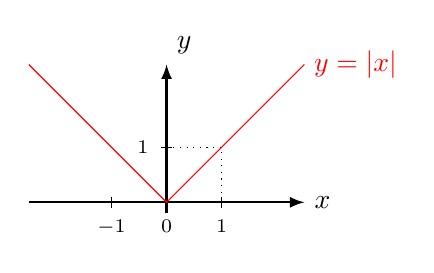
\begin{tikzpicture}[scale=.7]
\def \xa {-1};
\def \xb {1};
\def \ya {0};
\def \yb {1};
% Achsen zeichnen
\draw[-latex,thick] (\xa-1.5,0) -- (\xb+1.5,0) node[right] {$x$};
\draw[-latex,thick] (0,\ya-.2) -- (0,\yb+1.5) node[above right] {$y$};
% Achsen beschriften
\foreach \x in {\xa,...,\xb}
\draw (\x,-.1) -- (\x,.1) node[below=5pt] {$\scriptstyle\x$};
\foreach \y in {1,...,\yb}
\draw (-.1,\y) -- (.1,\y) node[left=5pt] {$\scriptstyle\y$};

\draw [dotted](0,1) -- (1,1) -- (1,0);

\draw [red] (2.5,2.5) node[right]{$y=|x|$} -- (0,0) -- (-2.5,2.5);
\end{tikzpicture}\\
Vorzeichenfunktion $sgn(x):= \begin{cases}
1 \quad x>0\\
0 \quad x=0\\
-1 \quad x<0
\end{cases}$
\subparagraph{Diskussion:} Es gilt:
\begin{enumerate}
\item $|a-b|$ = „Abstand der Zahlen $a$ und $b$ auf der Zahlengeraden“\\
\begin{tikzpicture}[scale=.7]
\draw [-latex] (-7,1.5) -- (0.5,1.5);
\draw (-5.5,1.25) node[below]{$a$} -- (-5.5,1.75);
\draw (-0.5,1.25) node[below]{$b$}-- (-0.5,1.75);
\draw [latex-latex, red](-5.5,2.5) -- (-0.5,2.5) node[pos=.5, above] {$|a-b|$};
\end{tikzpicture}\\
(speziell: $|a|$ = „Abstand von $a$ zum Ursprung“)
\item $a = |a| \cdot sgn (a)$
\item $|a|=|-a|, |ab|=|a|\cdot |b|, \left|\frac{a}{b}\right|=\frac{|a|}{|b|}$ (falls $b\not = 0$)
\item $|a \pm b| \leq |a| + |b|$ (\emph{Dreiecksungleichung}) für alle $a,b \in \mathbb{R}$
\end{enumerate}
\paragraph{Lösung von Ungleichung}
\subparagraph{Bsp. 14:} (Ungleichung mit Beträgen)\\
Gesucht sei die Lösungmenge $L$ der reellen Zahlen, die die Ungleichung $|x-1|<3+\frac{1}{2}x$ (*) erfüllen.
\begin{itemize}
\item kritische Stelle(n): Nullstellen des Terms innerhalb der Betragsstriche d.h. $x=1 \curvearrowright$ Fallunterscheidung\\
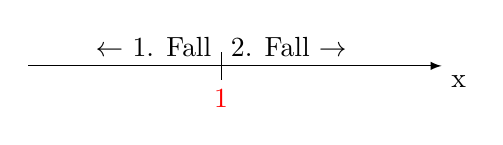
\begin{tikzpicture}[scale=.7]
\draw [-latex] (-7,1.5) -- (0.5,1.5) node[below right]{x};
\draw (-3.5,1.25) node[below]{$\color{red}1$} -- (-3.5,1.75);
\node at (-3.5,1.5) [above left] {$\leftarrow$ 1. Fall};
\node at (-3.5,1.5) [above right] {2. Fall $\rightarrow$};
\end{tikzpicture}
\item 1. Fall: $x-1<0$ d.h. $x<1$\\
in (*): \\
$\tred{-}(x-1)<3+\frac{1}{2}x \Leftrightarrow \\
-\frac{3}{2}x<2 \Leftrightarrow \\
\resultul{x>-\frac{4}{3}}$\\
$\curvearrowright L_1=\left\lbrace x|(x<1) \wedge x>\frac{4}{3}\right\rbrace = \left(-\frac{4}{3},1\right)$
\item 2. Fall $x-1 \geq 0$ d.h. $x\geq 1$\\
in (*):\\
$x-1< 3+ \frac{1}{2}x \Leftrightarrow\\
\frac{1}{2}x<4 \Leftrightarrow\\
\resultul{x<8}$\\
$\curvearrowright L_2 = \{ x| (x\geq 1) \wedge (x <8)\}=[1,8)$
\item $\Rightarrow L = L_1 \cup L_2 = \resultul{\left(-\frac{4}{3},8\right)}$
\end{itemize}
\subparagraph{Bsp. 15:} (Ungleichung mit gebrochen rationalen Termen)\\
$\frac{x}{x+1}<1$ (*)
\begin{itemize}
\item kritische Stelle(n): Nenner-Nullstellen, hier: $x=-1$.\\
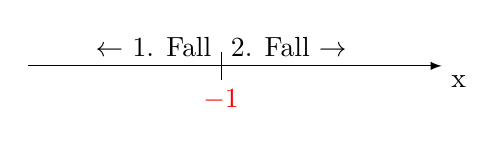
\begin{tikzpicture}[scale=.7]
\draw [-latex] (-7,1.5) -- (0.5,1.5) node[below right]{x};
\draw (-3.5,1.25) node[below]{$\color{red}-1$} -- (-3.5,1.75);
\node at (-3.5,1.5) [above left] {$\leftarrow$ 1. Fall};
\node at (-3.5,1.5) [above right] {2. Fall $\rightarrow$};
\end{tikzpicture}
\item 1. Fall: $x<-1$\\
in (*):\\
$\Leftrightarrow x>x+1 \Leftrightarrow 0>1$ (Widerspruch)\\
$L_1=\emptyset$.
\item 2. Fall: $x > -1$\\
in (*):\\
$\Leftrightarrow x < x+1 \Leftrightarrow 0<1$ (wahre Aussage)\\
$L_2=\{x|x>-1\}=(-1,\infty)$
\item $\Rightarrow L = L_1 \cup L_2 = \resultul{(-1,\infty)}$
\end{itemize}

\subparagraph{Bsp. 16:} (quadratische Ungleichungen)\\
$x^2+3x<10 \Leftrightarrow$ \\
$\left( x+\frac{3}{3}\right)^2-\frac{9}{4}<10 \Leftrightarrow$ (vereinfacht durch quadratische Ergännzung)\\
$\left( x+\frac{3}{2}\right)^2<\frac{49}{4} \Leftrightarrow\\
\left|x+\frac{3}{2}\right|<\frac{7}{2} \Leftrightarrow$ (Äquivalenz siehe Übung) \\
$\frac{-7}{2}<x+\frac{3}{2}<\frac{7}{2} \Leftrightarrow\\
-5<x<2$\\
$L=\resultul{(-5,2)}$\medskip\\
Bemerkung:\\
In vielen Fällen ist auch ein graphischer Lösungsansatz möglich. Dabei sind geeignete Schnittpunkte ($\widehat{=}$Gleichung) exakt rechnerisch zu ermitteln, ausschließend Ungleichheitszeichen betrachten.

\paragraph{in Bsp. 16:} \parskp
$x^2+3x<10 \qquad \Leftrightarrow \qquad \underbrace{x_2+3x-10}_{=f(x)}\tred{<}0$\\
Nullstellen von $f(x)$: \\
$x^2+3x-10=0$\\
$x_{1,2}=-\frac{3}{2}\pm \sqrt{\frac{9}{4}+10}=\begin{cases}
-5\\
2
\end{cases}$\\
$\curvearrowright$ Grobskizze von $y=f(x)$ (Parabel, nach oben geöffnet)\\
\begin{tikzpicture}[scale=.75]
\draw [-latex] (-6,0) -- (3,0) node [right]{$x$};
\draw [-latex] (0,-.25) -- (0,5) node [right] {$y$};
\begin{scope}[shift={(-1.5,-1.5)}]
\node at (0,0) {};
\draw[domain=-6:6,smooth] plot (\x,{1/8*\x*\x});
\end{scope}
\draw (-5,0.25) -- (-5,-0.25) node[below]{$-5$};
\draw (2,0.25) -- (2,-0.25) node[below]{$2$};
\draw [red] (-5,0.1) -- (2,0.1);
\end{tikzpicture}\\
$\tred{\curvearrowright} L=(-5,2)$

\paragraph{Schranken und Grenzen}
\begin{itemize}
\item Eine Menge $M\subseteq \mathbb{R}$ heißt nach oben beschränkt, wenn es eine obere Schranke gibt, vgl. \ref{sec:Mengen}. Man kann zeigen, dass es bei diesen Ordnungsrelationen ($\leq$) auf $\mathbb{R}$ dann auch eine kleinste obere Schranke (\emph{Supremum, $sup\;M$, $s=max \; M$} falls $s \in M$)
\item Analog: nach \emph{unten beschränkt, Infimum, Minimum}.
\item Falls $M$ \emph{nicht} nach oben beschränkt ist, d.h. es gilt:\\
$\exists a \in \mathbb{R}\quad \forall x \in M\quad x \leq a = \forall a \in \mathbb{R} \quad \exists x \in M \quad x >a$, dann Schreibweise $\boxed{sup\; M := \infty}$
\item Analog: in $\boxed{inf\; M:= - \infty}$ falls $M$ \emph{nicht} nach unten beschränkt.
\item $M$ heißt \emph{beschränkt}, falls $M$ nach oben und unten beschränkt ist.
\end{itemize} 

\subparagraph{Bsp. 17:} \parskp
$M=\left\lbrace 1+\frac{1}{n}\;|\;n\in \mathbb{N}^*\right\rbrace$
\begin{itemize}
\item \emph{obere Schranken}: $\pi$, $2300$, $7$, $2,01$ usw.\\
kleinste obere Schranke: $sup \; M = 2= max \; M$
\item \emph{untere Schranken}: $-31$, $0$, $0,99$ usw.\\
größte untere Schranke: $inf\; M =1$ ($1 \not \in M \curvearrowright min \; M$ existiert nicht)
\end{itemize}
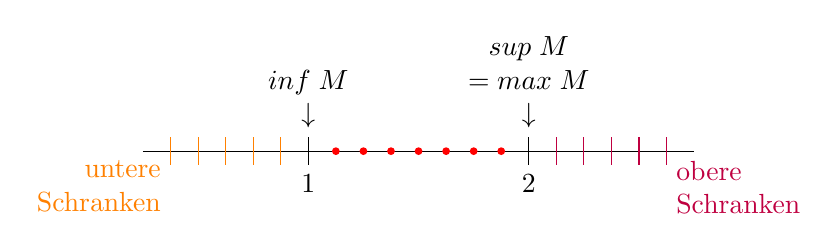
\begin{tikzpicture}[scale=.7]
\draw (-1,0) -- (9,0){};
\draw (2,0.25) node[above, align=center]{$inf\;M$\\$\downarrow$} -- (2,-0.25) node[below]{$1$};
\draw (6,0.25) node[above, align=center]{$sup\;M$\\$=max\; M$\\$\downarrow$} -- (6,-0.25) node[below]{$2$};
\foreach \x in {2.5,3,...,5.5}{
\fill [red] (\x,0) circle[radius=2pt];
}
\foreach \x in {-.5,0,...,1.5}{
\draw [orange](\x,0.25) -- (\x,-0.25);
\draw [purple] (\x+7,0.25) -- (\x+7,-0.25);
}
\node [below left, orange, align=right] at (-0.5,0) {untere \\Schranken};
\node [below right, purple, align=left] at (8.5,0) {obere \\Schranken};
\end{tikzpicture}

\subsection{Komplexe Zahlen}

\paragraph{Motivation:} z.B. $\boxed{x^2+1=0}$ ($\Leftrightarrow x^2=-1$) im Bereich der reellen Zahlen nicht lösbar.
$\curvearrowright$ Zahlenbereichserweiterung

\subsubsection{Begriff, Rechenregeln}

Die Menge $\mathbb{C}$ der komplexen Zahlen ist eine Obermenge der Menge der reellen Zahlen mit folgenden Eigenschaften:
\begin{enumerate}
\item $\mathbb{C}$ enthält eine Zahl $i$ mit $\boxed{i^2=-1}$ (oft auch mit $j$ bezeichnet)
\item Jede komplexe Zahl $z$ lässt sich in der Form $\boxed{z=x+i\cdot y} \quad (x,y \in \mathbb{R})$ darstellen.\\
Dabei $x=Re(z)$ (Realteil) und $y=Im(z)$ (Imaginärteil)
\item Auf $\mathbb{C}$ werden die Operationen $+$ (Addition) und $\cdot$ (Multiplikation) wie folgt erklärt: \\
Sei $z_1=x_1+i\cdot y_1$, $z_2=x_2+i\cdot y_2$ Dann gilt: \\
$z_1+z_2:= (x_1+x_2)+ i (y_1+y_2)$\\
$z_1\cdot z_2 := (x_1 x_2-y_1 y_2)+i (x_1 y_2 + x_2 y_1)$\\
Die Menge $\mathbb{C}$ wird mit diesen Operationen zum \emph{Körper der komplexen Zahlen}. Die arithmetischen Operationen erfolgen unter Beachtung von $i^2=-1$ wie im Reellen.
\item Auf $\mathbb{C}$ gibt es keine natürliche Ordnungsrelation.\\
Veranschaulichung: \emph{GAUSSsche Zahlenebene}\\
Zahl $z \leftrightarrow$ Punkt $(x,y) \leftrightarrow$ Vektor $\overrightarrow{OP}$\\
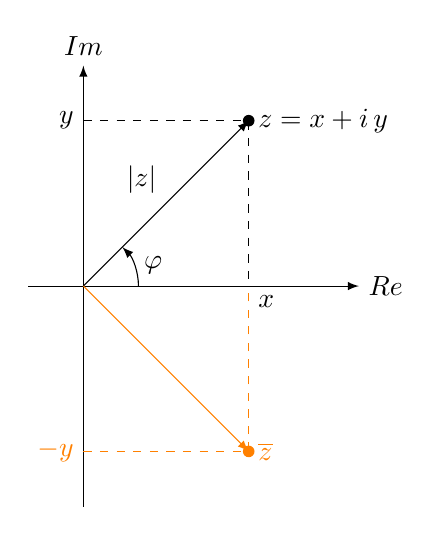
\begin{tikzpicture}[scale=.7]
\draw [-latex] (-1,0) -- (5,0) node[right]{$Re$};
\draw [-latex] (0,-4) -- (0,4) node[above]{$Im$};

\draw [dashed] (0,3) node[left]{$y$} -- (3,3) -- (3,0) node [below right]{$x$};
\fill (3,3) circle[radius=3pt] node [right]{$z=x+i\, y$};
\draw [-latex] (0,0) -- (3,3) node[pos=0.5, above left]{$|z|$};

\draw [-latex] (0,0) ++(0:1) arc (0:45:1) node [pos=.5, right]{$\varphi$};

\draw [dashed, orange] (0,-3) node[left]{$-y$} --(3,-3) -- (3,0);
\fill [orange] (3,-3) circle[radius=3pt] node [right]{$\overline{z}$};

\draw [-latex, orange] (0,0) -- (3,-3) ;
\end{tikzpicture}
\begin{itemize}
\item \emph{Betrag} von $z$: \\
$|z|=\sqrt{x^2+y^2}$
\item Hauptarrgument von $z$: orientierter Winkel zwischen positiver x-Achse und $\overrightarrow{OP}$ (gemessen auf kürzestem Wege)\\
$Arg(z):= \varphi \qquad (-\pi < \varphi \leq \pi )$
\item zu $z$ konjugiert komplexe Zahl $\overline{z}:$\\
$\overline{z} := x - i \cdot y$
\end{itemize}
\end{enumerate}

\paragraph{Diskussion:}
\begin{itemize}
\item Falls nicht notwendig kürzester Weg gewählt wird: Argument $arg(z)= Arg(z) + 2\pi k \quad (k \in \mathbb{Z})$\\
z.B. $z=1-i \quad : \quad Arg(z)=-45^{\circ}=-\frac{\pi}{4}$, ein (Neben-)argument bspw. $arg(z)=315^{\circ}$
\item Berechnung von $Arg(z) \; (z \not = 0)$: $cos \varphi = \frac{x}{|z|}$, $sin\varphi = \frac{y}{|z|}$\\
$\boxed{ Arg (z)= \begin{cases}
+arccos \frac{x}{|z|}\qquad \text{falls } y \leq 0\\
-arccos \frac{x}{|z|} \qquad \text{falls } y < 0
\end{cases}}$
\end{itemize}
\subparagraph{Bsp. 18:} \parskp
$z_1 = 3 + 4i$, $z_2=-12-5i$\\
\begin{tikzpicture}[scale=.5]
\draw [-latex] (-13,0) -- (4,0) node[right]{$Re$};
\draw [-latex] (0,-6) -- (0,5) node[above]{$Im$};

\draw [dashed] (0,4) node[left]{$4$} -- (3,4) -- (3,0) node [below]{$3$};
\fill (3,4) circle[radius=3pt] node [right]{$z_1$};
\draw [-latex] (0,0) -- (3,4) ;

\draw [dashed] (0,-5) node[right]{$-5$} -- (-12,-5) -- (-12,0) node [above]{$-12$};
\fill (-12,-5) circle[radius=3pt] node [left]{$z_2$};
\draw [-latex] (0,0) -- (-12,-5) ;

\draw [-latex, orange] (0,0) ++(0:1) arc (0:53:1) node [pos=.5, right]{$\varphi_1$};
\draw [-latex, purple] (0,0) ++(0:1) arc (0:-146:2) node [pos=.5, below]{$\varphi_2$};
\end{tikzpicture}
\begin{enumerate}[label=\alph*.)]
\item Betrag und Hauptargument\\
$|z_1|=\sqrt{3^2+4^2}=5$\\
$\varphi_1 = Arg(z_1) = arccos \frac{3}{5} \approx 53,13 ^{\circ}$\\
$|z_2| = 13$\\
$\varphi_2=Arg(z_2) = - arccos -\frac{12}{13} \approx -157,38 ^{\circ}$
\item Arithmetische Operationen:\\
$z_1 + z_2 = -9 - i$\\
$z_1 - z_2 = 15 + 9 i$\\
$z_1 \cdot z_2 = -16 - 63 i$\\
$\frac{z_1}{z_2}=\frac{z_1 \cdot \overline{z_2}}{z_2 \cdot \overline{z_2}}=\frac{z_1 \cdot \overline{z_2}}{|z_2|^2}=-\frac{56}{169}-\frac{33}{169}i$
\end{enumerate}

\subsubsection{Darstellungsformen komplexer Zahlen}
\begin{itemize}
\item Trigonometrische Darstellung
\item EULERsche Form
\item exponentielle Darstellung
\end{itemize}
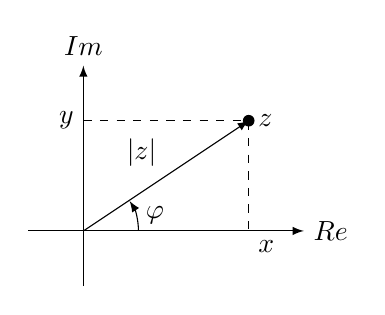
\begin{tikzpicture}[scale=.7]
\draw [-latex] (-1,0) -- (4,0) node[right]{$Re$};
\draw [-latex] (0,-1) -- (0,3) node[above]{$Im$};

\draw [dashed] (0,2) node[left]{$y$} -- (3,2) -- (3,0) node [below right]{$x$};
\fill (3,2) circle[radius=3pt] node [right]{$z$};
\draw [-latex] (0,0) -- (3,2) node[pos=0.5, above left]{$|z|$};

\draw [-latex] (0,0) ++(0:1) arc (0:33:1) node [pos=.5, right]{$\varphi$};

\end{tikzpicture}\\
$\boxed{z=x+iy}$ \qquad (\emph{arithmetische Darstellung})\\
$x=|z|\cdot cos \varphi$\\
$y=|z|\cdot sin \varphi$\\
$\curvearrowright \boxed{z=|z|\cdot (cos\varphi + i\; sin \varphi)}$ \qquad (\emph{trigonometrische Darstellung})\\
(und $\varphi=arg\; z$, meist $\varphi = Arg \; z$)
\subparagraph{Diskussion:} \parskp
$z_1= |z_1|\cdot (cos \varphi_1 + i \; sin \varphi_1)$\\
$z_2= |z_2|\cdot (cos \varphi_2 + i \; sin \varphi_2)$\medskip\\
$z_1 \cdot z_2 = |z_1| \cdot |z_2| \cdot ( \underbrace{(cos\varphi_1 \; cos \varphi_2 - sin\varphi_1 \; sin \varphi_2)}_{\cos(\varphi_1+\varphi_2)}+i\underbrace{(sin \varphi_1 \; cos \varphi_2 + sin \varphi_2 \; cos \varphi_1)}_{\sin(\varphi_1+\varphi_2)})$\\
$\boxed{z_1 \cdot z_2 = |z_1| \cdot |z_2| \cdot(\cos(\varphi_1+\varphi_2)+i\; \sin(\varphi_1+\varphi_2))}$\\
Folgerung:\\
$\boxed{|z_1\cdot z_2| = |z_1| \cdot |z_2|}\\
\boxed{arg(z_1\cdot z_2)=arg(z_1)+arg(z_2)}$\\
Analog:\\
$\boxed{\left|\frac{z_1}{z_2}\right| = \frac{|z_1|}{|z_2|} \qquad (z_2 \not = 0)} \\
\boxed{arg\left(\frac{z_1}{z_2}\right) = arg(z_1) - arg (z_2)}$\\
Es ist also sinnvoll zu definieren:
\paragraph{Def. 10:} \parskp
$\boxed{e^{i\varphi}=cos\varphi+i\; sin \varphi}$ \qquad (\emph{EULERsche Form})
\subparagraph{Diskussion:}
\begin{enumerate}
\item \emph{Exponentielle Darstellung} von z: $\boxed{z=|z|\cdot e^{i\varphi}}$
\item Wegen der obigen Formeln bleiben für diese Darstellung die vom Reellen bekannnten Potenzgesetze gültig.\\
Insbesondere gilt die Formel von MOIVRE: \\
$\boxed{z^n=\left(|z|\cdot e^{i\varphi}\right)^n=|z|^n\cdot e^{i\varphi n}=|z|^n(\cos(n\varphi)+i\; \sin(n \varphi)}$
\end{enumerate}

\subparagraph{Bsp. 19:}
\begin{enumerate}
[label=\alph*.)]
\item $z_1=\underbrace{3+4i}_{\tgreen{arithmetisch}}=\underbrace{5\cdot (cos 53,13^{\circ}+i\; \sin(53,13^{\circ})}_{\tgreen{trigonemetrisch}}=\underbrace{5\cdot e^{i\cdot 53,13^{\circ}}}_{\tgreen{exponentiell}}$\\
$z_2=-12-5i=13\cdot (\cos(-157,38^{\circ}+i\; 
-157,38^{\circ}))=13\cdot e^{-i\cdot 157,38^{\circ}}$
\item $z=-1+i$, gesucht: $z^{12}$\\
$|z|=\sqrt{2}$, $Arg(z)=arccos\left(-\frac{1}{\sqrt{2}}\right)=135^{\circ}=\frac{3}{4}\pi$\\
$z=\sqrt{2}\cdot e^{i\cdot \frac{3}{4}\pi}\Rightarrow z^12=\left(\sqrt{2}\cdot e^{i\frac{3}{4}\pi}\right)=2^6\cdot e^{i\frac{3}{4}\pi \cdot 12}=64 \cdot e ^{i\cdot 9 \pi}=64\cdot e^{i\pi}$\\
arithmetische Darstellung: $z^{12}=64\cdot (cos\pi+i\; sin\pi)=\resultul{-64}$
\end{enumerate}

\subsubsection{Spezielle Gleichungen}
Quadratische Gleichung: $z^2+p\cdot z+q=0 \qquad (p,q \in \mathbb{R})$

quadratische Ergänzung: $\left(z+\frac{p}{2}\right)^2=\frac{p^2}{4}-q$

1. Fall: $\frac{p}{2}-q \geq 0 \curvearrowright z_{1/2}=-\frac{p}{2}\pm \sqrt{\frac{p^2}{4}-q}$

2. Fall: $\frac{p^2}{4}-q < 0 \\
\Leftrightarrow \left(z+\frac{p}{2}\right)^2+\overbrace{\underbrace{q-\frac{p^2}{4}}_{>0}}^{\widehat=a^2}=0 \\
\Leftrightarrow \left(\left(z+\frac{p}{2}\right)+i\cdot a\right)\cdot \left(\left(p+\frac{p}{2}\right)-i\cdot a\right)=0\\
\Leftrightarrow \boxed{z_{1,2}=-\frac{p}{2}\pm i \sqrt{q-\frac{p^2}{4}}}$\\
praktisches Vorgehen:

Lösungsformel aus dem ersten Fall stets anwenden, im Fall 2 Formal $\sqrt{-1}=\pm i$.

\subparagraph{Bsp. 20:}\parskp
$z^2+28z+200=0$\\
$z_{1,2}=-14\pm \sqrt{-4}=\resultul{-14\pm 2i}$

\paragraph{Kreisteilungsgleichung:} \parskp
$\boxed{z^n=b}, b\in \mathbb{C}, n\in \mathbb{N}^*$\\
Lösung:
\begin{itemize}
\item $b$ exponentiell darstellen: $b=|b| \cdot e ^{i\beta} \quad , \beta = Arg(b)$
\item Gleichung besitzt $n$ Lösungen $\boxed{z_k=\sqrt[n]{|b|}\cdot e^{i\frac{\beta+k\cdot 360^{\circ}}{n}}}$ \qquad mit $k=0,1,...,n-1$
\end{itemize}
zum Beweis: \\
Ansatz: $z=r\cdot e^{i\varphi}$\\
$z^n=\torange{r^n}\cdot e^{i\tgreen{\varphi n}}=\torange{|b|} \cdot e^{i\tgreen{\beta}}$\\
Zwei Gleichungen stimmen überein, wenn jeweils der \torange{Betrag} gleich und \tgreen{Winkel} bis auf ein vielfaches von $\pi$ gleich ist.
\begin{enumerate}
\item $r^n=|b| \curvearrowright r = \sqrt[n]{|b|}$
\item $\varphi \cdot n = \beta + k \cdot 360^{\circ} \qquad (k \in \mathbb{Z})\\
\curvearrowright \varphi = \frac{\beta + k \cdot 360^{\circ}}{n}$\qquad (nur $n$ verschiedene Argumente)
\end{enumerate}
Beispiele:
\begin{enumerate}[label=\alph*.)]
\item $z^3=1=1\cdot e^{i\cdot 0}$\\
$z_k=1^{\frac{1}{3}}\cdot e^{i\frac{0+k\cdot 2 \pi}{3}} \qquad (k=0,1,2)$\\
$z_0=e^{i\cdot 0}=\resultul{1}\\
z_1= e^{\frac{2}{3}\pi}=\cos(\frac{2}{3}\pi)+i\; \sin(\frac{2}{3}\pi)=\resultul{-\frac{1}{2}+\frac{1}{2}\sqrt{3}i}\\
z_2=e^{i\frac{4}{3}\pi}=\cos(\frac{4}{3}\pi)+i\; \sin(\frac{4}{3}\pi)=\resultul{-\frac{1}{2}-\frac{1}{2}\sqrt{3}i}$\\
Allgemein: Lösungen der Gleichung $z^n=b$ teilen Kreis mit Radius $\sqrt[n]{|b|}$ um $0$ in $n$ gleiche Teile.\\
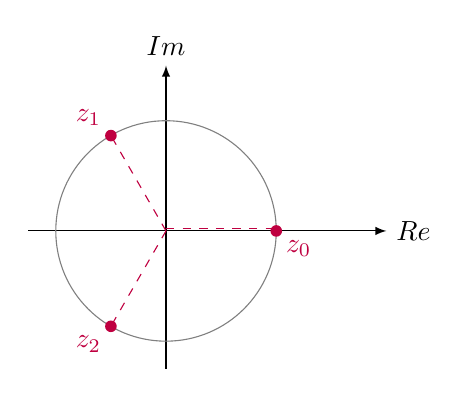
\begin{tikzpicture}[scale=.7]
\draw [-latex] (-2.5,0) -- (4,0) node[right]{$Re$};
\draw [-latex] (0,-2.5) -- (0,3) node[above]{$Im$};

\draw [gray] (0,0) circle[radius=2];
\fill [purple](2,0) circle[radius=3pt] node[below right]{$z_0$};
\fill [purple](-1,1.73) circle[radius=3pt] node[above left]{$z_1$};
\fill [purple](-1,-1.73) circle[radius=3pt] node[below left]{$z_2$};
\draw [purple, dashed] (0,0.05) -- (2,0.05);
\draw [purple, dashed] (0,0) -- (-1,-1.73);
\draw [purple, dashed] (0,0) -- (-1,1.73);
\end{tikzpicture}
\item $z^4=-16=16\cdot e^{i\cdot \pi}$\\
$z_k=2\cdot e^{i\frac{\pi + k \cdot 2\pi}{4}} \qquad (k=0,1,2,3,4)$\\
$z_0=2\cdot e^{i\frac{\pi}{4}}=\resultul{\sqrt{2}+\sqrt{2}i}\\
z_1=2\cdot e^{i\frac{3\pi}{4}}=\resultul{-\sqrt{2}+\sqrt{2}i}\\
z_2=2\cdot e^{-i\frac{3\pi}{4}}=\resultul{-\sqrt{2}-\sqrt{2}i}\\
z_3=2\cdot e^{-i\frac{\pi}{4}}=\resultul{\sqrt{2}-\sqrt{2}i}$\\
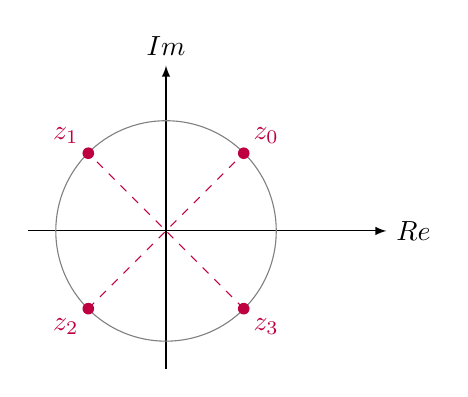
\begin{tikzpicture}[scale=.7]
\draw [-latex] (-2.5,0) -- (4,0) node[right]{$Re$};
\draw [-latex] (0,-2.5) -- (0,3) node[above]{$Im$};

\def \xa{1.41};

\draw [gray] (0,0) circle[radius=2];
\fill [purple](\xa,\xa) circle[radius=3pt] node[above right]{$z_0$};
\fill [purple](-\xa,\xa) circle[radius=3pt] node[above left]{$z_1$};
\fill [purple](-\xa,-\xa) circle[radius=3pt] node[below left]{$z_2$};
\fill [purple](\xa,-\xa) circle[radius=3pt] node[below right]{$z_3$};
\draw [purple, dashed] (-\xa,-\xa) -- (\xa, \xa);
\draw [purple, dashed] (\xa,-\xa) -- (-\xa, \xa);
\end{tikzpicture}
\end{enumerate}
Anwendung: \\
Faktorisierung des Polynoms $p(x)=x^4+16$
\begin{align*}
x^4+16 &= (x-z_0)\cdot(x-z_1)\cdot(x-z_2)\cdot(x-z_3)\\
&= (x-\sqrt{2}-\sqrt{2}i)\cdot (x-\sqrt{2}+\sqrt{2}i)\cdot (x+\sqrt{2}-\sqrt{2}i) \cdot (x+\sqrt{2}+\sqrt{2}i)\\
&= (x^2-2\sqrt{2}x+4)(x^2+2\sqrt{2}x+4)
\end{align*}

\subsubsection{Anwendung im Wechselstromkreis}
\begin{enumerate}
\item Spule: \\
Stromstärke $I=I_m\cdot \tred{(}\cos(\omega t) \tred{+ i \; \sin(\omega t))}$\\
Spannung $U=\omega \cdot L\cdot I_m \cdot \tred{(}\cos(\omega t +\frac{\pi}{2}) \tred{+ i \; \sin(\omega t  +\frac{\pi}{2}))}$\\
\tred{(formale Ergänzung zu komplexer Größe)}\\
$\curvearrowright I=I_m \cdot e^{i\omega t}, \; U=I_m\cdot \omega \cdot L \cdot e^{i(\omega t+\frac{\pi}{2}}=\underbrace{I_m\cdot \omega \cdot L \cdot e^{i\omega t}}_{I\cdot \omega \cdot L}\cdot \underbrace{e^{i\frac{\pi}{2}}}_i$\\
$R=\frac{U}{I}\curvearrowright \boxed{R_L=\omega \cdot L \cdot i}$ (\emph{induktiver Widerstand})
\item Kondensator: \\
$\boxed{R_C=\frac{1}{\omega \cdot C \cdot i}}$ (\emph{kapazitiver Widerstand})
\end{enumerate}
Bezeichnung in E-Technik:\\
$Z:= R_ges = R+i\cdot X$\\
Wirkwiderstand $R$, Blindwiderstand $X$, Scheinwiderstand $|Z|$, Leitwert $Y=\frac{1}{Z}$

\subparagraph{Bsp. 22:} \parskp
\begin{tikzpicture}[scale=.4]
\draw  (-6,1.5) rectangle (-5,-1.5);
\draw (-1.5,-1.5) -- (-1.5,-3.5);
\draw (-1,-1.5) -- (-1,-3.5);

\draw  plot[smooth, tension=1] coordinates {(1.5,-2.5) (2,-2) (2.5,-2.5)};
\draw  plot[smooth, tension=1] coordinates {(2.5,-2.5) (3,-2) (3.5,-2.5)};
\draw  plot[smooth, tension=1] coordinates {(3.5,-2.5) (4,-2) (4.5,-2.5)};
\draw  plot[smooth, tension=1] coordinates {(4.5,-2.5) (5,-2) (5.5,-2.5)};
\draw (-5.5,-1.5) -- (-5.5,-2.5) -- (-1.5,-2.5);
\draw (-1,-2.5) -- (1.5,-2.5);
\draw (5.5,-2.5) -- (7,-2.5) -- (7,3.5) -- (1.7,3.5);
\draw (0.3,3.5) -- (-5.5,3.5) -- (-5.5,1.5);

\draw (1.5,3.5) circle[radius=.2];
\draw (0.5,3.5) circle[radius=.2];
\node at (1,4.5) {$\sim 220V, 50Hz$};
\node at (-6,0) [left]{$R$};
\node at (-1.25,-4.5) {$C$};
\node at (3.5,-3.5) {$L$};
\end{tikzpicture}\\
$R=100 \Omega, C = 20 \mu F=20\cdot 10^{-6}\frac{As}{V}, L=1H=1 \frac{Vs}{A}, \omega = 2\pi \cdot \underbrace{50 \frac{1}{s}}_{f}$\\
Gesucht ist der Gesamtwiderstand $Z$.\\
$Z=R + R_C + R_L = R+i \omega L + \frac{1}{i \omega C}=R+i(\omega L - \frac{1}{\omega C})$\\
$Z=(\tblue{100}+\torange{155,04}i)\Omega = \tgreen{184,44} \cdot e^{i\cdot \tpurple{57,17^{\circ}}}\Omega$\\
$\curvearrowright$ \\
Wirkwiderstand: $\tblue{Re(Z)}=100 \Omega$\\
Blindwiderstand: $\torange{Im(Z)}=155,04 \Omega$\\
Scheinwiderstand: $\tgreen{|Z|}=184,44 \Omega$\\
Phasenverschiebung: $\tpurple{Arg(Z)}=57,17^{\circ}$